\section{Pianificazione}
Nella pianificazione, il responsabile suddividerà il lavoro in attività e le assegnerà a ciascun membro del team.
Lo scopo è quello di mostrare come verrà svolto il lavoro, valutare i progressi nel progetto e anticipare i problemi che potrebbero sorgere preparando così delle soluzioni a tali problemi. 
La pianificazione di progetto è stata organizzata seguendo le scadenze presenti nella sezione § 1.6 Scadenze.
Lo sviluppo del progetto è stato suddiviso nelle seguenti 4 fasi: 
\begin{itemize}
	\item Analisi;
	\item Progettazione Architetturale;
	\item Progettazione di Dettaglio e Codifica;
	\item Validazione e Collaudo;
\end{itemize}
Ogni fase sarà suddivisa in periodi più brevi all'interno dei quali verranno elencate le diverse attività che il gruppo \Gruppo{} svolgerà.


\subsection{Analisi}

\subsubsection{Periodo 1} 
Dal 2019-11-15 al 2019-11-29\\
In questo periodo, che parte dalla formazione del gruppo e termina con la scelta del capitolato C5, abbiamo affrontato le seguenti tematiche al fine di porre le basi per il lavoro che dovevamo affrontare:\\
\begin{itemize}
	\item \textbf{Discussione capitolati:} per prima cosa abbiamo studiato individualmente e in seguito discusso durante gli incontri tutti i capitolati proposti, questo ha posto le basi per la stesura del documento \SdF{} e ci ha indirizzati verso la scelta del capitolato che avremmo affrontato;
	\item \textbf{Spartizione e studio dei ruoli:} a ogni membro del gruppo è stato assegnato il ruolo che svolgerà nella fase di Analisi;
	\item \textbf{Definizione degli strumenti:} Abbiamo discusso e definito le tecnologie che avremmo usato per affrontare la fase di Analisi;
	\item \textbf{Pianificazione milestone fase di Analisi:} Abbiamo discusso e fissato delle milestone da rispettare per completare la fase di Analisi entro le scadenze imposteci.
\end{itemize}
\subsubsection{Periodo 2} 
Dal 2019-11-30 al 2019-12-31\\
Questo periodo inizia con la scelta definitiva del capitolato C5.\\
Dopo la scelta abbiamo focalizzato le risorse del gruppo sui seguenti punti:
\begin{itemize}
	\item \textbf{Normazione: }Abbiamo definito le regole per la stesura dei documenti e per l'utilizzo delle tecnologie identificate in precedenza;
	\item \textbf{Approfondimento capitolati: }Abbiamo ulteriormente discusso tutti i capitolati in modo da terminare lo studio di fattibilità e focalizzato la nostra analisi su quello scelto in modo da predisporre le basi per l'analisi dei requisiti;
	\item \textbf{Prima definizione dei casi d'uso};
	\item \textbf{Determinazione standard di qualità: }Abbiamo definito le nostre strategie per garantire la qualità di processo e di prodotto;
	\item \textbf{Verifica: }Verifica dell'andamento del team in relazione alle tempistiche e allo svolgimento dei compiti assegnati.
\end{itemize}
\subsubsection{Periodo 3}
 Dal 2020-01-01 al 2020-01-14\\
 Questo periodo si estende fino alla data ultima di consegna per affrontare la revisione dei requisiti a cui il nostro gruppo ha deciso di partecipare.\\
 \begin{itemize}
	\item \textbf{Normazione: }Ulteriori approfondimenti alle regole per la stesura dei documenti e per l'utilizzo delle tecnologie;
	\item \textbf{Approfondimento delle tecnologie: }Abbiamo ampliato le nostre conoscenze sulle tecnologie richieste dal capitolato per essere svolto;
	\item \textbf{Analisi dei requisiti: } Studio dei requisiti e raffinamento dei casi d'uso;
	\item \textbf{Pianificazione attività: }Pianificazione del lavoro da svolgere nelle fasi successive a quella di Analisi;
	\item \textbf{Verifica: }Verifica dell'andamento del team in relazione alle tempistiche e allo svolgimento dei compiti assegnati.

 \end{itemize}
\subsubsection{Periodo 4} 
Dal 2020-01-15 al 2020-01-20\\
In questo periodo che parte dalla consegna dei documenti per la revisione dei requisiti alla presentazione pubblica della proposta il gruppo consolida il lavoro svolto in vista delle successive fasi e della discussione per la quale serve una presentazione;
\begin{itemize}
	\item \textbf{Consolidamento:} Ogni membro si prende del tempo per ripassare tutto il lavoro svolto e per studiare il necessario per affrontare al meglio le fasi successive;
	\item \textbf{Preparazione per la Revisione dei Requisiti:} Il gruppo produce il materiale necessario da esporre alla presentazione pubblica della nostra proposta.
\end{itemize}

	\newpage
	% Inizia la pagina orientata orizzontalmente
	\begin{landscape}
	 % Ora la pagina e' in orizzontale!
	\subsubsection{Diagramma di Gantt delle attività}
	\pagestyle{empty}
	\begin{figure}[h]
		\caption{Diagramma di Gantt delle attività di Analisi}
		\begin{center}	
			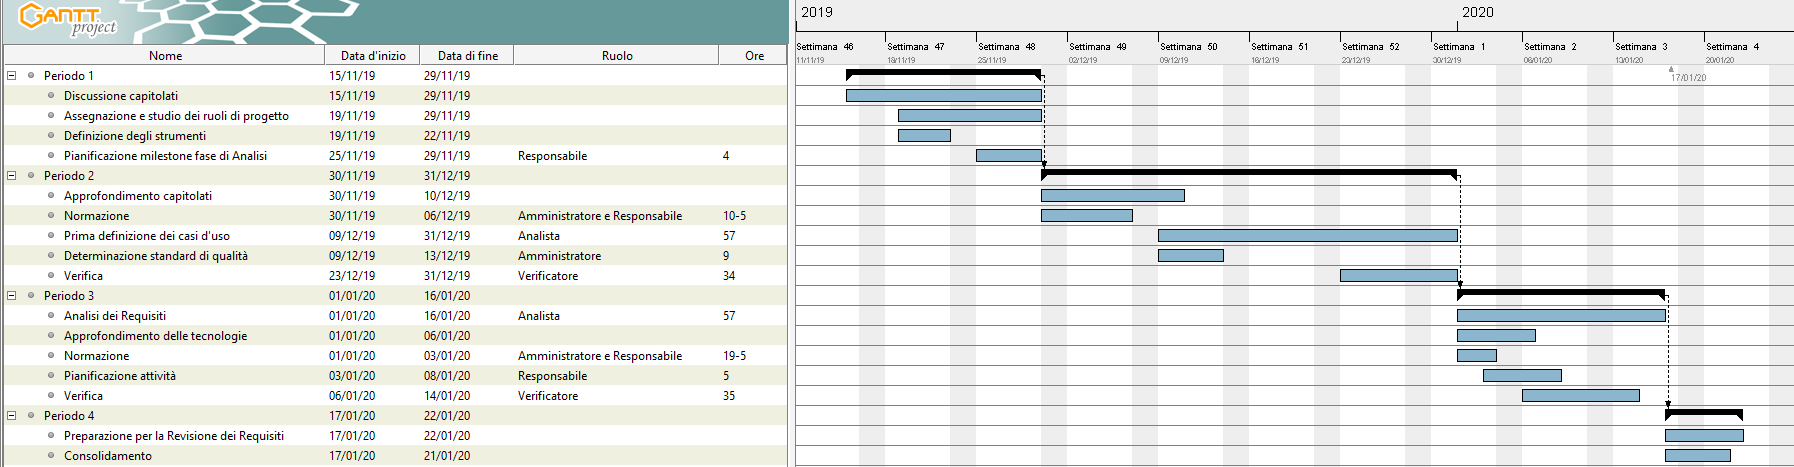
\includegraphics[scale=0.50]{Sezioni/DiagrammiGantt/Analisi.png}
		\end{center}
		
	\end{figure}
	 \end{landscape}

\clearpage
\subsection{Progettazione Architetturale}
Periodo: dal 2020-01-22 al 2020-03-15.
\\Inizia al termine dell'Analisi dei Requisiti e finisce con la data di consegna della Revisione di Progettazione.
\\In questa fase viene definita una soluzione architetturale in modo da soddisfare i requisiti individuati nel periodo di Analisi dei Requisiti.

\subsubsection{Periodo 1} 
Dal 2020-01-22 al 2020-02-11
\begin{itemize}
	\item \textbf{Normazione};
	\item \textbf{Analisi dei requisiti};
	\item \textbf{Pianificazione attività};
	\item \textbf{Approfondimento delle tecnologie};
	\item \textbf{Verifica}.
\end{itemize}
\subsubsection{Periodo 2} 
Dal 2020-02-12 al 2020-03-08
\begin{itemize}
	\item \textbf{Studio delle tecnologie:} IAAS Kubernetes\ap{G} o PaaS\ap{G}, Openshift\ap{G} o Rancher\ap{G}, LDAP\ap{G} e GPS\ap{G};
	\item \textbf{Normazione};
	\item \textbf{Miglioramento standard di qualità};
	\item \textbf{Technology Baseline\ap{G}:} redazione della Technology baseline;
	\item \textbf{Proof of Concept\ap{G}:} rappresentazione della Baseline\ap{G};
	\item \textbf{Codifica:} viene codificato il Proof of Concept;
	\item \textbf{Verifica}.
\end{itemize}
\subsubsection{Periodo 3} 
Dal 2020-03-09 al 2020-03-15
\begin{itemize}
	\item \textbf{Consolidamento};
	\item \textbf{Preparazione per la Revisione di Progettazione}.
\end{itemize}

\newpage
% Inizia la pagina orientata orizzontalmente
\begin{landscape}
	% Ora la pagina e' in orizzontale!
	\subsubsection{Diagramma di Gantt delle attività}
	\pagestyle{empty}
	\begin{figure}[h]
		\caption{Diagramma di Gantt delle attività di Progettazione}
		\begin{center}	
			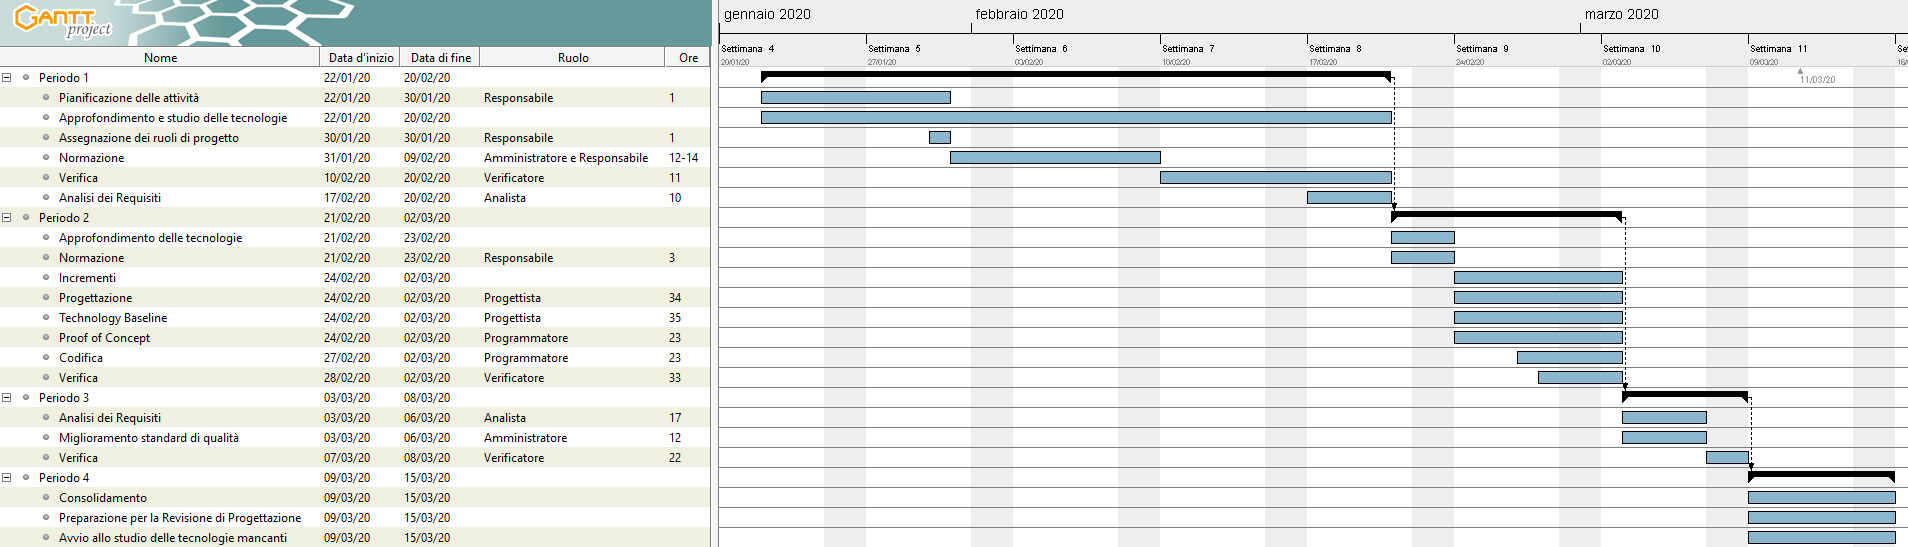
\includegraphics[scale=1.6]{Sezioni/DiagrammiGantt/ProgettazioneArchitetturale.png}
		\end{center}
		
	\end{figure}
\end{landscape}

\subsection{Progettazione di Dettaglio e Codifica}
Dal 2020-03-16 al 2020-04-19\\
Inizia al termine della Progettazione Architetturale e finisce con la data di consegna della Revisione di Qualifica.\\
In questa fase si definisce nel dettaglio e si implementa l'architettura logica costruita nella fase di Progettazione Architetturale.\\


\subsubsection{Periodo 1} 
Dal 2020-03-16 al 2020-03-27\\
\begin{itemize}
	\item \textbf{Approfondimento delle tecnologie};
	\item \textbf{Normazione};
	\item \textbf{Pianificazione delle attività};
	\item \textbf{Progettazione};
	\item \textbf{Codifica:} Implementazione dei requisiti di base identificati per ottenere un sistema stabile;
	\item \textbf{Manuali:} Stesura manuale utente e manuale manutentore in relazione alle funzionalità di base del sistema.
\end{itemize}
\subsubsection{Periodo 2} 
Dal 2020-03-28 al 2020-04-08\\
\begin{itemize}
	\item \textbf{Implementazione della Product Baseline:} seguendo le specifiche della Technology Baseline;
	\item \textbf{Codifica incrementale:} Aggiunta di requisiti al sistema tramite incrementi;
	\item \textbf{Incremento e verifica:} Verifiche ed eventuali aggiunte al lavoro svolto in precedenza;
	\item \textbf{Manuali:} Aggiunta nel manuale utente e nel manuale manutentore delle funzionalità inserite incrementalmente nel sistema;
\end{itemize}
\subsubsection{Periodo 3}
Dal 2020-04-09 al 2020-04-12\\
\begin{itemize}
	\item \textbf{Primo rilascio del prodotto};
	\item \textbf{Verifica:} Verifica dell'andamento del team in relazione alle tempistiche e allo svolgimento dei compiti assegnati;
\end{itemize}
\subsubsection{Periodo 4} 
Dal 2020-04-13 al 2020-04-19\\
\begin{itemize}
	\item \textbf{Consolidamento};
	\item \textbf{Preparazione per la Revisione di Qualifica}.
\end{itemize}

\newpage
% Inizia la pagina orientata orizzontalmente
\begin{landscape}
	% Ora la pagina e' in orizzontale!
	\subsubsection{Diagramma di Gantt delle attività}
	\pagestyle{empty}
	\begin{figure}[h]
			\caption{Diagramma di Gantt delle attività di Progettazione di Dettaglio e Codifica}
		\begin{center}	
				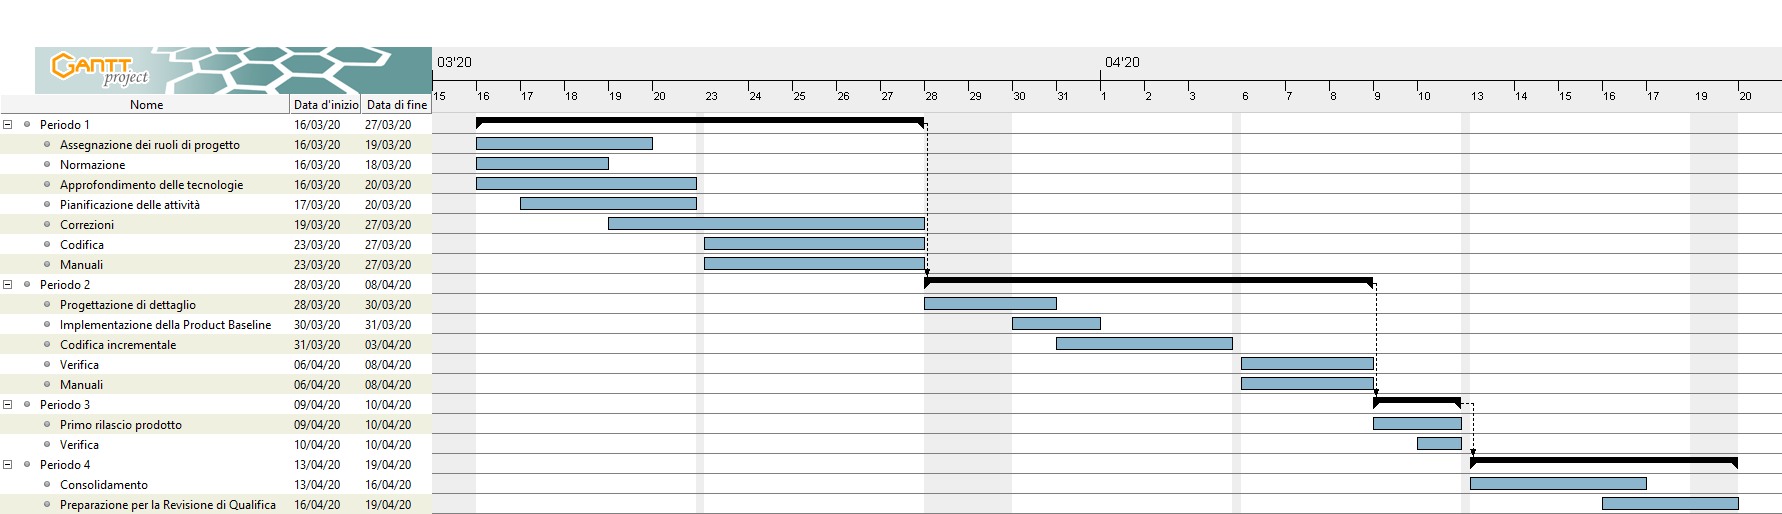
\includegraphics[scale=0.5]{Sezioni/DiagrammiGantt/ProgettazioneDiDettaglio.png}	
		\end{center}
		
	\end{figure}
\end{landscape}

\subsection{Validazione e Collaudo}
Inizia al termine della Progettazione di Dettaglio e Codifica e finisce con la data di consegna della Revisione di Accettazione.
\\In questo fase vengono definite le attività che servono per verificare che il prodotto corrisponde a quello desiderato dal cliente.
\subsubsection{Periodo 1} 
Dal 2020-04-21 al 2020-04-28
\begin{itemize}
	\item \textbf{Normazione};
	\item \textbf{Analisi dei requisiti};
	\item \textbf{Pianificazione attività};
	\item \textbf{Verifica}.
\end{itemize}
\subsubsection{Periodo 2} 
Dal 2020-04-29 al 2020-05-10
\begin{itemize}
	\item \textbf{Codifica:} verrà eseguito l'ultimo versionamento del prodotto;
	\item \textbf{Verifica:} verrà accertato che le esecuzioni delle attività siano esenti da errori;
	\item \textbf{Validazione:} verrà verificato se il prodotto realizzato sia conforme alle attese;
	\item \textbf{Scrittura dei manuali:} verrà eseguito il secondo versionamento del manuale Utente e del manuale Manutentore;
	\item \textbf{Collaudo:} vengono eseguiti gli ultimi test sul prodotto per verificare se le funzionalità rispettano i risultati attesi.
\end{itemize}
\subsubsection{Periodo 3} 
Dal 2020-05-11 al 2020-05-17
\begin{itemize}
	\item \textbf{Preparazione per la Revisione di Accettazione}.
\end{itemize}


\newpage
% Inizia la pagina orientata orizzontalmente
\begin{landscape}
	% Ora la pagina e' in orizzontale!
	\subsubsection{Diagramma di Gantt delle attività}
	\pagestyle{empty}
	\begin{figure}[h]
		\caption{Diagramma di Gantt delle attività di Validazione e Collaudo}
		\begin{center}	
			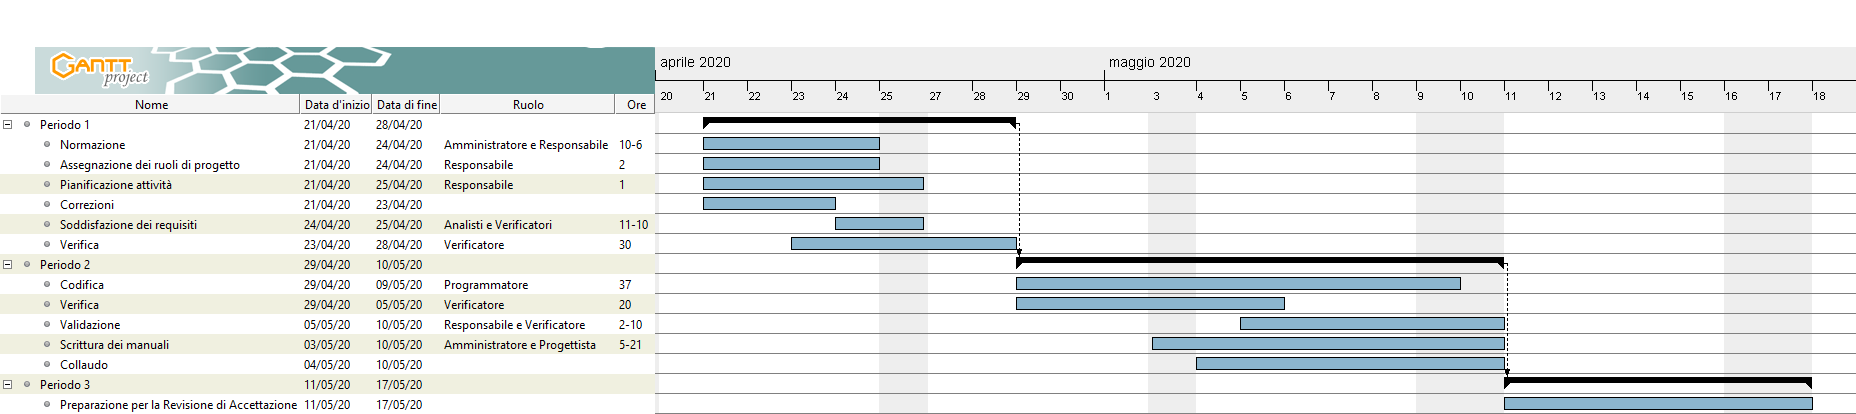
\includegraphics[scale=1.6]{Sezioni/DiagrammiGantt/Validazione.png}
		\end{center}
		
	\end{figure}
\end{landscape}